%
% related-work.tex
%
% Copyright (C) 2022 by Universidade Federal de Santa Catarina.
%
% GNSS Networks Based on Small Satellites
%
% This work is licensed under the Creative Commons Attribution-ShareAlike 4.0
% International License. To view a copy of this license,
% visit http://creativecommons.org/licenses/by-sa/4.0/.
%

%
% \brief Related works section.
%
% \author Gabriel Mariano Marcelino <gabriel.mm8@gmail.com>
%
% \version 0.0.0
%
% \date 2021/06/14
%

\section{Related Work} \label{sec:related-work}

\subsection{Current GNSS networks}

Atualmente existem N redes de GNSS em operação, X em fase de implantação e testes e Y redes em planejamento.

Abaixo, encontra-se uma descrição de cada uma dessas redes.

\subsubsection{GPS}

\cite{gps}

\subsubsection{GLONASS}

O GLONASS, sigla de \textit{Globalnaya navigatsionnaya sputnikovaya sistema} (ou Sistema de Navegação Global por Satélite) \cite{glonass}, é o sistema de GNSS criado e mantido pela Rússia.

GLONASS (Globalnaya Navigazionnaya Sputnikovaya Sistema, or Global Navigation Satellite System) is a global GNSS owned and operated by the Russian Federation. The fully operational system consists of 24+ satellites.

\subsubsection{Galileo}

O Galileo é o sistema de GNSS criado pela união europeia.

Galileo is a global GNSS owned and operated by the European Union. The EU declared the start of Galileo Initial Services in 2016 and plans to complete the system of 24+ satellites in 2021.

\subsubsection{BDS}

O \textit{BeiDou Navigation Satellite System}, ou BDS \cite{beidou}, é o sistema de GNSS chinês.

BeiDou, or BDS, is a global GNSS owned and operated by the People's Republic of China. BDS was formally commissioned in 2020. The operational system consists of 35 satellites. BDS was previously called Compass.



A \autoref{tab:networks-comparison} compara as principais características dos sistemas de GNSS apresentados acima.

\begin{table*}[!h]
    \centering
    \begin{tabular}{lcccccc}
        \toprule[1.5pt]
        \multirow{2}{*}{\textbf{Characteristic}} & \multicolumn{6}{c}{\textbf{Network}} \\
                                                 & \textbf{GPS} & \textbf{GLONASS} & \textbf{Galileo} & \textbf{BDS} & \textbf{QZSS} & \textbf{IRNSS} \\
        \midrule
        Coverage                         & Global            & Global                       & Global               & Global         & Local   & Local \\
        Country                          & United States     & Russia                       & European Union       & China          & Japan   & India \\
        Satellites                       & 32                & 24                           & 30                   & 30             &         &  \\
        Orbit                            &                   &                              &                      &                &         &  \\
        Altitude                         &                   &                              &                      &                &         &  \\
        \multirow{6}{*}{Frequency [MHz]} & 1575,42           & 1598,0625-1609,3125          & 1575,42              & 1561,098       & 1575,42 & 1176,45 \\
                                         & 1227,6            & 1242,9375-1251,6875          & 1176,45              & 1207,14        & 1227,6  &  \\
                                         & 1176,45           & 1202,025                     & 1207,14              & 1268,52        & 1176,45 &  \\
                                         &                   &                              & 1191,795             & 1575,42        & 1278,75 &  \\
                                         &                   &                              & 1275,75              & 1176,45        &         &  \\
                                         &                   &                              &                      & 1207,14        &         &  \\
        Bandwidth [MHz]                  & 15,345/11/12,5    &                              &                      &                &         &  \\
        Modulation                       &                   &                              &                      &                &         &  \\
        Precision                        &                   &                              &                      &                &         &  \\
        Status                           & Fully operational &                              &                      &                &         &  \\
        \bottomrule[1.5pt]
    \end{tabular}
    \caption{Comparison between the current operational GNSS networks.}
    \label{tab:networks-comparison}
\end{table*}

%        \multirow{6}{*}{Frequency [MHz]} & 1575,42 (L1 C/A)  & 1598,0625-1609,3125 (L1 C/A) & 1575,42 (E1)         & 1561,098 (B1l) & 1575,42 (L1 C/A/S) & 1176,45 (L5) \\
%                                         & 1227,6 (L2 C/P)   & 1242,9375-1251,6875 (L2 C/P) & 1176,45 (E5a)        & 1207,14 (B2l)  & 1227,6 (L2C)       &  \\
%                                         & 1176,45 (L5)      & 1202,025            (L3 OC)  & 1207,14 (E5b)        & 1268,52 (B3l)  & 1176,45 (L5)       &  \\
%                                         &                   &                              & 1191,795 (E5 AltBOC) & 1575,42 (B1C)  & 1278,75 (L6)       &  \\
%                                         &                   &                              & 1275,75 (E6)         & 1176,45 (B2a)  &                    &  \\
%                                         &                   &                              &                      & 1207,14 (B2b)  &                    &  \\

\subsection{Local networks}

.

\subsubsection{QZSS}

Quasi-Zenith Satellite System \cite{qzss}

QZSS is a regional GNSS owned by the Government of Japan and operated by QZS System Service Inc. (QSS). QZSS complements GPS to improve coverage in East Asia and Oceania. Japan declared the official start of QZSS services in 2018 with 4 operational satellites, and plans to expand the constellation to 7 satellites by 2023 for autonomous capability.

\subsubsection{IRNSS}

Indian Regional Navigation Satellite System \cite{irnss}

IRNSS is a regional GNSS owned and operated by the Government of India. IRNSS is an autonomous system designed to cover the Indian region and 1500 km around the Indian mainland. The system consists of 7 satellites. In 2016, India renamed IRNSS as the Navigation Indian Constellation (NavIC, meaning ``sailor'' or ``navigator'').

\subsection{Experimental GNSS networks}

\cite{aarestad2020}

\begin{figure}[!ht]
    \begin{center}
        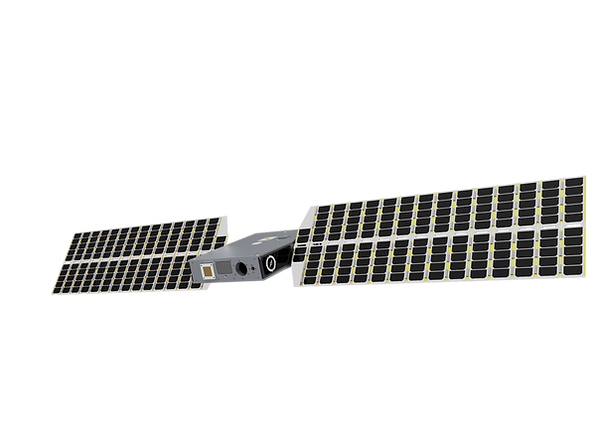
\includegraphics[width=\columnwidth]{figures/xona-satellite}
        \caption{Xona Space Systems conceptual satellite.}
        \label{fig:xona-satellite}
    \end{center}
\end{figure}
